\chapter{Random Matrices and Families of L Functions}\label{ch:06}

In spring 1972 Hugh Montgomery visited the Institute for Advanced Study and, over tea, described to Freeman Dyson the function $1-(\sin\pi u/\pi u)^2$ that he had found governing the pair correlation of zeros of the Riemann zeta function. Dyson recognised it at once as the pair correlation of eigenvalues of a random Hermitian matrix from the Gaussian unitary ensemble. That conversation set the agenda for half a century: the conjecture, supported by theorems for restricted test functions and by extensive computation, that zeros of $L$ functions have the local statistics of eigenvalues of random matrices from compact classical groups. This chapter develops the theory, from the Weyl integration formula to the Katz and Sarnak symmetry types, low lying zeros and the Keating and Snaith moment conjectures. Throughout we keep two random matrix limits apart: the Sato Tate limit, in which a fixed compact group of small rank governs Frobenius classes at varying primes, and the Katz and Sarnak limit, in which groups of growing dimension govern the zeros near a fixed point.

\section{Haar measure and the Weyl integration formula}\label{sec:ch6weyl}

Every compact group $K$ carries a unique left and right invariant probability measure, the Haar measure\index{Haar measure} (Chapter~\ref{ch:04}). When $K$ is a connected Lie group, the integral $\int_Kf\,dh$ of a class function $f$ (one constant on conjugacy classes) reduces to an integral over a maximal torus $T$, because every element of $K$ is conjugate into $T$ and two elements of $T$ are conjugate in $K$ precisely when they lie in one orbit of the Weyl group $W=N(T)/T$. The density of the pushforward to $T/W$ is given by Weyl's formula \cite{weyl1925}.\index{Weyl integration formula}

\begin{theorem}[Weyl integration formula]\label{thm:ch6weyl}
Let $K$ be a compact connected Lie group with maximal torus $T$, Weyl group $W$ and set of roots $\Phi$. For every continuous class function $f$,
\[
\int_Kf\,dh=\frac{1}{|W|}\int_Tf(t)\prod_{\alpha\in\Phi}\bigl(1-\alpha(t)\bigr)\,dt ,
\]
where $dt$ is Haar probability measure on $T$.
\end{theorem}

For the unitary group $\mathrm{U}(N)$, with eigenvalues $e^{i\theta_1},\dots,e^{i\theta_N}$, the formula gives the joint density
\[
\frac{1}{(2\pi)^NN!}\prod_{j<k}\bigl|e^{i\theta_j}-e^{i\theta_k}\bigr|^2
\]
on $[0,2\pi)^N$. This is the circular unitary ensemble (CUE). For the compact symplectic group $\USp(2g)$, eigenvalues come in pairs $e^{\pm i\theta_j}$ with $\theta_j\in[0,\pi]$, and the joint density of $(\theta_1,\dots,\theta_g)$ is
\begin{equation}\label{eq:ch6usp}
\frac{2^{g^2}}{g!\,\pi^g}\prod_{j<k}(\cos\theta_j-\cos\theta_k)^2\prod_{j=1}^g\sin^2\theta_j .
\end{equation}
For the even and odd orthogonal groups the factor $\prod\sin^2\theta_j$ is replaced by $1$ and by $\prod\sin^2(\theta_j/2)$, with different constants \cite{katzsarnak1999}. The factor $\prod_{j<k}(\cos\theta_j-\cos\theta_k)^2$, common to the three groups, is eigenvalue repulsion; the single product, which depends on the group, is the interaction with the symmetry point $\theta=0$, and it is this factor that the low lying zeros of Section~\ref{sec:ch6ils} detect. For $\SU(2)=\USp(2)$, Chapter~\ref{ch:04} derives the density from the geometry of the three sphere; here is a proof through Gaussian vectors.

\begin{proposition}\label{prop:ch6su2}
Let $A$ be Haar distributed in $\SU(2)$, with eigenvalues $e^{\pm i\theta}$, $\theta\in[0,\pi]$. Then $\theta$ has density $\frac2\pi\sin^2\theta$, and $x=\tr A=2\cos\theta$ has the semicircle density $\frac{1}{2\pi}\sqrt{4-x^2}$ on $[-2,2]$.
\end{proposition}

\begin{proof}
As in Chapter~\ref{ch:04}, Haar measure on $\SU(2)$ is uniform measure on the unit quaternions $S^3\subset\R^4$ and $\tr A=2u$ with $u$ the first coordinate, so $u$ has the law of $Z_1/(Z_1^2+Z_2^2+Z_3^2+Z_4^2)^{1/2}$ for independent standard Gaussian $Z_j$, and $u^2$ has the Beta$(\frac12,\frac32)$ law. Since $u$ is symmetric, its density is $\frac2\pi\sqrt{1-u^2}$ on $[-1,1]$, and the substitutions $u=\cos\theta$ and $x=2u$ give both claims.
\end{proof}

This agrees with \eqref{eq:ch6usp} for $g=1$. The semicircle is both the Sato Tate law and the Wigner law of large random matrices, but here it is the exact law of the trace of a $2\times2$ matrix. For large $N$, the traces of powers of a Haar unitary matrix are nearly independent Gaussians.

\begin{theorem}[Diaconis and Shahshahani \cite{diaconisshahshahani1994}]\label{thm:ch6ds}
Let $U_N$ be Haar distributed in $\mathrm{U}(N)$ and let $Z_1,Z_2,\dots$ be independent standard complex Gaussian variables, $\E|Z_j|^2=1$. For each fixed $k$,
\[
\bigl(\tr U_N,\tr U_N^2,\dots,\tr U_N^k\bigr)\Rightarrow\bigl(Z_1,\sqrt2\,Z_2,\dots,\sqrt k\,Z_k\bigr)\qquad(N\to\infty).
\]
Moreover, for nonnegative integers $m_j,n_j$ with $N\ge\max(\sum jm_j,\sum jn_j)$, the mixed moments $\E\prod_j(\tr U_N^j)^{m_j}\overline{(\tr U_N^j)}^{n_j}$ equal those of the Gaussian limit exactly, namely $\delta_{m,n}\prod_jj^{m_j}m_j!$.
\end{theorem}

The proof uses power sum symmetric functions and Schur orthogonality; Diaconis and Evans \cite{diaconisevans2001} extended the central limit theorem to linear statistics $\sum_jf(\theta_j)$ with $f$ in the Sobolev space of order one half. Diaconis and Shahshahani also treat the orthogonal and symplectic groups, whose traces are real and whose Gaussian limits acquire a mean shift: for $\USp(2N)$, $\E\tr U^j=-1$ for even $j\le2N$ and $\E\tr U^j=0$ otherwise. As a check we drew $4000$ Haar unitary matrices with $N=50$; the sample means of $|\tr U^j|^2/j$ were $1.001$, $0.994$, $1.013$ for $j=1,2,3$, each with standard error about $0.016$, and the correlation between $|\tr U|^2$ and $|\tr U^2|^2$ was $-0.012$. Heuristically, through the explicit formula, the Gaussian behaviour of $\tr U^j$ mirrors the near independence of the contributions $\tr A_p^j\log p/p^{j/2}$ of distinct prime powers.

\section{Montgomery, Dyson and Odlyzko}\label{sec:ch6mont}

Assume the Riemann hypothesis and write the nontrivial zeros of $\zeta$ as $\frac12+i\gamma$. Near height $T$ the zeros have density $\frac{1}{2\pi}\log\frac{T}{2\pi}$. We list the ordinates in the upper half plane with multiplicity, $0<\gamma_1\le\gamma_2\le\cdots$, and unfold them by $\tilde\gamma_j=\frac{\gamma_j}{2\pi}\log\frac{\gamma_j}{2\pi e}$, the main term of the number of zeros up to height $\gamma_j$, so that the mean spacing of the $\tilde\gamma_j$ tends to one.\index{pair correlation}

\begin{theorem}[Montgomery \cite{montgomery1973}]\label{thm:ch6mont}
Assume the Riemann hypothesis. Let $f$ be a Schwartz function whose Fourier transform $\hat f(\xi)=\int f(x)e^{-2\pi ix\xi}dx$ is supported in $(-1,1)$. Then, as $T\to\infty$,
\[
\frac{1}{N(T)}\sum_{\substack{j\ne l\\ \gamma_j,\gamma_l\le T}}f(\tilde\gamma_j-\tilde\gamma_l)\longrightarrow\int_{-\infty}^{\infty}f(u)\Bigl(1-\Bigl(\frac{\sin\pi u}{\pi u}\Bigr)^2\Bigr)du ,
\]
where $N(T)$ is the number of zeros with $0<\gamma\le T$, counted with multiplicity.
\end{theorem}

The pair correlation conjecture, that the limit holds for all Schwartz $f$, remains open. The function $1-(\sin\pi u/\pi u)^2$ is the limiting pair correlation of the CUE. Rudnick and Sarnak \cite{rudnicksarnak1996} extended Montgomery's theorem to all $n$ level correlations and to cuspidal automorphic $L$ functions of $\GL_m$, again for restricted support, assuming the Riemann hypothesis for the $L$ function and, for larger $m$, an auxiliary hypothesis on the coefficients at prime powers (Theorem~\ref{thm:09brs} in Chapter~\ref{ch:09b} gives the precise statement). In that range the bulk statistics, those of zeros at large height, do not depend on the $L$ function and agree with those of the CUE.

Odlyzko \cite{odlyzko1987} computed large blocks of zeros near the $10^{12}$th zero and later near the $10^{20}$th, with an algorithm developed with Schönhage \cite{odlyzkoschonhage1988}. The nearest neighbour spacings agree closely with Gaudin's spacing law for the unitary ensemble \cite{gaudin1961}. The small systematic deviations that remain are lower order effects: Bogomolny, Bohigas, Leboeuf and Monastra \cite{bblm2006} matched them with Haar unitary matrices of an effective size proportional to $\log\frac{T}{2\pi}$. Figure~\ref{fig:ch06_spacing} shows the random matrix experiment: spacings of $400$ independent CUE matrices of size $200$, against the Wigner surmise $\frac{32}{\pi^2}s^2e^{-4s^2/\pi}$, the exact spacing law for $2\times2$ matrices of the Gaussian unitary ensemble and a close approximation to Gaudin's law.\index{Wigner surmise} The sample variance of the spacings is $0.180$, the Gaudin value, against $\frac{3\pi}{8}-1\approx0.178$ for the surmise and $1$ for Poisson spacings; repetitions of the experiment fluctuate by about $0.001$, so a single run of this size separates the Gaudin law from the surmise only marginally.

\begin{figure}[t]\centering
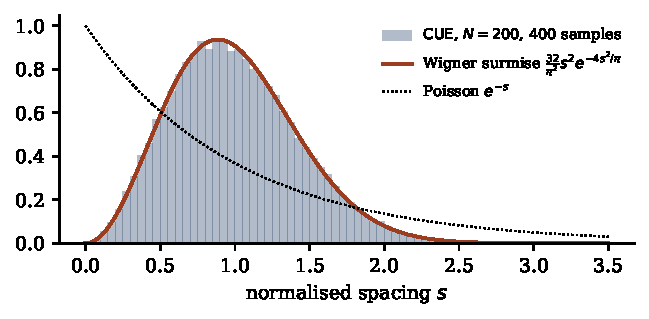
\includegraphics[width=\textwidth]{figs/ch06_spacing.pdf}
\caption{Nearest neighbour spacings of the eigenvalue angles of $400$ Haar unitary matrices of size $N=200$, scaled by $N/2\pi$ to have mean one ($80{,}000$ spacings), with the Wigner surmise $\frac{32}{\pi^2}s^2e^{-4s^2/\pi}$ for $\beta=2$ and the Poisson density $e^{-s}$. The quadratic vanishing at $s=0$ is eigenvalue repulsion.}\label{fig:ch06_spacing}
\end{figure}

\section{The Katz and Sarnak philosophy}\label{sec:ch6ks}

Katz and Sarnak \cite{katzsarnak1999,katzsarnak1999b} found that, unlike the bulk statistics, the statistics of zeros near the central point $s=\frac12$, averaged over a family, distinguish families, and that the distinction is by the symmetry type of a classical group.\index{Katz and Sarnak philosophy}

In function fields the analogous statements are theorems. Let $C$ be a smooth projective curve of genus $g$ over $\mathbb{F}_q$. Its zeta function is
\[
Z(C,u)=\frac{P_C(u)}{(1-u)(1-qu)},\qquad P_C(u)=\det\bigl(1-u\,F\mid H^1\bigr),
\]
a polynomial of degree $2g$. By Weil's theorem its roots have absolute value $q^{-1/2}$, so $P_C(q^{-1/2}u)=\det(1-u\,\vartheta_C)$ for a conjugacy class $\vartheta_C$ in $\USp(2g)$, the unitarised Frobenius; an eigenvalue $e^{i\theta}$ of $\vartheta_C$ corresponds to the zeros $s=\frac12+i(\theta+2\pi m)/\log q$, $m\in\Z$, of $Z(C,q^{-s})$. Let $C$ vary in an algebraic family, for instance the hyperelliptic curves $y^2=f(x)$ with $q$ odd and $f$ squarefree of degree $2g+1$. Deligne's equidistribution theorem \cite{deligne1980} says that as $q\to\infty$ the classes $\vartheta_C$ become equidistributed for the Haar measure of a maximal compact subgroup of the geometric monodromy group of the family, here all of $\USp(2g)$. Letting first $q\to\infty$ and then $g\to\infty$, Katz and Sarnak proved for many families over function fields that the low lying zeros follow one of a few limiting laws, labelled by the symmetry types\index{symmetry type}
\[
\mathrm{U},\quad\USp,\quad\mathrm{SO(even)},\quad\mathrm{SO(odd)},\quad\mathrm{O}.
\]

Over number fields the symmetry type of a family is conjectural: Dirichlet $L$ functions $L(s,\chi)$ with $\chi$ ranging over primitive characters of a large modulus are unitary; quadratic Dirichlet characters $\chi_d$ are symplectic; holomorphic newforms of weight $k$ and level $N$ with $N\to\infty$ are orthogonal, splitting into $\mathrm{SO(even)}$ and $\mathrm{SO(odd)}$ according to the root number; quadratic twists of a fixed elliptic curve are orthogonal, again split by root number. For several of these families the prediction has been proved, for test functions of restricted support only and assuming the generalized Riemann hypothesis where needed; Section~\ref{sec:ch6ils} treats the newforms.

To make this precise, fix an even Schwartz function $\phi$ whose Fourier transform $\hat\phi$ has compact support, so that $\phi$ extends to an entire function. For an $L$ function $L(s,f)$ in the unitary normalisation of Chapter~\ref{ch:02} (centre $\frac12$), with analytic conductor $c_f$ and nontrivial zeros $\frac12+i\gamma_f$, counted with multiplicity and not assumed to be real, the one level density\index{one level density} is $D(f;\phi)=\sum_{\gamma_f}\phi\bigl(\frac{\gamma_f}{2\pi}\log c_f\bigr)$, scaled so that the mean spacing near the central point is one. For a classical group $G(N)$ of $N\times N$ matrices, the analogous statistic $\sum_j\phi(N\theta_j/2\pi)$ of a Haar random matrix, summed over its $N$ eigenvalue angles $\theta_j\in(-\pi,\pi]$, has expectation converging to $\int\phi(x)W(G)(x)\,dx$ as $N\to\infty$, where, with $\operatorname{si}(x)=\frac{\sin2\pi x}{2\pi x}$,
\begin{align*}
W(\mathrm{U})&=1, & W(\USp)&=1-\operatorname{si},\\
W(\mathrm{SO(even)})&=1+\operatorname{si}, & W(\mathrm{SO(odd)})&=1-\operatorname{si}+\delta_0,\\
W(\mathrm{O})&=1+\tfrac12\delta_0.
\end{align*}
In Fourier terms, with $\hat W$ in the sense of distributions and $\mathbb{I}=\mathbb{I}_{[-1,1]}$ the indicator, $\hat W(\mathrm{U})=\delta_0$ and
\begin{align*}
\hat W(\USp)&=\delta_0-\tfrac12\mathbb{I}, & \hat W(\mathrm{SO(even)})&=\delta_0+\tfrac12\mathbb{I},\\
\hat W(\mathrm{O})&=\delta_0+\tfrac12, & \hat W(\mathrm{SO(odd)})&=\delta_0+1-\tfrac12\mathbb{I}.
\end{align*}
Figure~\ref{fig:ch06_onelevel} plots the densities of the first four types. The three orthogonal densities have the same Fourier transform on $(-1,1)$, so test functions with $\operatorname{supp}\hat\phi\subset(-1,1)$ cannot tell them apart; only support beyond $[-1,1]$ separates them.

\begin{figure}[t]\centering
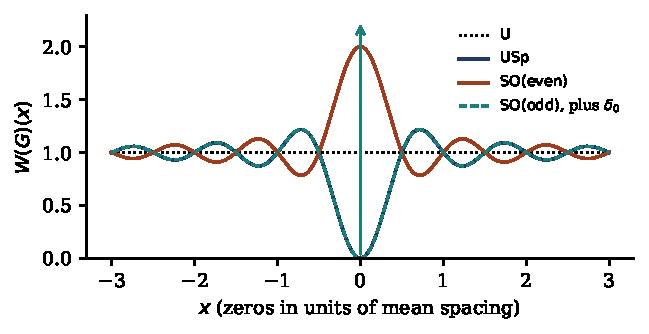
\includegraphics[width=\textwidth]{figs/ch06_onelevel.pdf}
\caption{One level densities $W(G)(x)$ of the symmetry types $\mathrm{U}$, $\USp$, $\mathrm{SO(even)}$ and $\mathrm{SO(odd)}$, with $x$ in units of the mean spacing. The symplectic density vanishes quadratically at the origin; the even orthogonal density equals $2$ there, twice the unitary value; the odd orthogonal density is the symplectic one plus a unit point mass at the origin (arrow), from the eigenvalue forced at $1$. The full orthogonal density $1+\frac12\delta_0$, not drawn, is the average of the even and odd orthogonal densities.}\label{fig:ch06_onelevel}
\end{figure}

\section{Low lying zeros of modular forms}\label{sec:ch6ils}

The first theorem over $\Q$ that separates the orthogonal types is due to Iwaniec, Luo and Sarnak \cite{ils2000}, and its method is the template for later work.\index{low lying zeros}

\begin{theorem}[Iwaniec, Luo and Sarnak \cite{ils2000}]\label{thm:ch6ils}
Assume the generalized Riemann hypothesis for the $L$ functions of holomorphic newforms and for Dirichlet $L$ functions. Fix an even weight $k$, let $N$ run through squarefree integers, and let $H_k^*(N)$ be the set of holomorphic newforms of weight $k$ and level $N$, with analytic conductor $c_f=k^2N$, and $H_k^\pm(N)$ the subsets of root number $\pm1$. Let $\phi$ be an even Schwartz function with $\operatorname{supp}\hat\phi\subset(-2,2)$. Then
\[
\lim_{N\to\infty}\frac{1}{|H_k^\pm(N)|}\sum_{f\in H_k^\pm(N)}D(f;\phi)=\int\phi(x)W(\mathrm{SO}(\pm))(x)\,dx,
\]
where $\mathrm{SO}(+)=\mathrm{SO(even)}$ and $\mathrm{SO}(-)=\mathrm{SO(odd)}$; for the full family $H_k^*(N)$ the limit is $\int\phi\,W(\mathrm{O})$. For $\operatorname{supp}\hat\phi\subset(-1,1)$ the limits for $H_k^\pm(N)$ hold as $kN\to\infty$, without the hypothesis on Dirichlet $L$ functions.
\end{theorem}

Averaging also over the weight brings in level one, where the root number is $i^k$: under the same hypotheses Iwaniec, Luo and Sarnak prove these limits for the forms of weight $k\le K$ and fixed level as $K\to\infty$, with support in $(-2,2)$. For the level one forms of weight $k\le K$, not split by root number and weighted by the harmonic weights of the Petersson formula, proportional to $L(1,\Sym^2f)^{-1}$, they prove the orthogonal limit $\int\phi\,W(\mathrm{O})$ for $\operatorname{supp}\hat\phi\subset(-2,2)$ unconditionally.

The proof starts from the explicit formula, which for $f\in H_k^*(N)$, assuming also the Riemann hypothesis for $L(s,\Sym^2f)$, gives\index{explicit formula}
\[
D(f;\phi)=\hat\phi(0)+\tfrac12\phi(0)-\frac{2}{\log c_f}\sum_{p\nmid N}\lambda_f(p)\hat\phi\Bigl(\frac{\log p}{\log c_f}\Bigr)\frac{\log p}{\sqrt p}+O\Bigl(\frac{\log\log3kN}{\log c_f}\Bigr),
\]
with $\lambda_f(p)=x_p\in[-2,2]$ the normalised Hecke eigenvalues. The term $\frac12\phi(0)$ comes from the prime squares. The coefficient of $p^{-2s}$ in $-L'/L(s,f)$ is $(\lambda_f(p)^2-2)\log p=(\lambda_f(p^2)-1)\log p$; the part with $\lambda_f(p^2)$ is negligible (this is where the Riemann hypothesis for the symmetric square enters; Iwaniec, Luo and Sarnak note that on average over the family Petersson's formula replaces it, for the same support, so the theorem does not assume it), and the constant $-1$, summed by the prime number theorem, gives $\frac12\phi(0)$. For a symplectic family such as $L(s,\chi_d)$ the coefficient is $\chi_d(p)^2\log p=\log p$ and the same sum gives $-\frac12\phi(0)$. This is the arithmetic shadow of the mean shift $\E\tr U^2=\pm1$ in orthogonal and symplectic groups. Petersson's formula then averages the sum over primes. For $\operatorname{supp}\hat\phi\subset(-1,1)$ its Kloosterman terms are negligible, so the prime sum averages to $o(1)$ and the average of $D(f;\phi)$ is $\hat\phi(0)+\frac12\phi(0)$ for both root numbers, in keeping with the agreement of the three orthogonal densities there. Beyond $(-1,1)$ these terms, evaluated with the generalized Riemann hypothesis for Dirichlet $L$ functions, contribute main terms of opposite signs to the two root numbers, through $\varepsilon_f=i^k\mu(N)\sqrt N\lambda_f(N)$; they cancel in the full family, and they are what separates $\mathrm{SO(even)}$ from $\mathrm{SO(odd)}$.

Under the generalized Riemann hypothesis the zeros are real, so if $\phi\ge0$ and $\phi(0)=1$ the order of vanishing of $L(s,f)$ at $\frac12$ is at most $D(f;\phi)$. Averaging over the family and choosing $\phi$ well, Iwaniec, Luo and Sarnak deduce that for all large squarefree $N$ more than $\frac9{16}$ of the forms in $H_k^+(N)$ have $L(\frac12,f)\ne0$ and more than $\frac{15}{16}$ of those in $H_k^-(N)$ have $L'(\frac12,f)\ne0$; the extension of the support beyond $(-1,1)$ is essential for these constants. For test functions of unrestricted support the Katz and Sarnak prediction is not known for any family over a number field.

\subsection{Why the central point sees the group}

For a self dual $L$ function the zeros are symmetric about $s=\frac12$, just as the eigenvalues of orthogonal and symplectic matrices come in pairs $e^{\pm i\theta}$; a matrix in $\mathrm{SO}(2N+1)$ always has the eigenvalue $1$, as an $L$ function of root number $-1$ vanishes at $\frac12$. Away from the symmetry point all groups look unitary; near it, the factor $\prod\sin^2\theta_j$ or $\prod\sin^2(\theta_j/2)$ in the Weyl density decides whether eigenvalues are repelled from $1$. Low lying zeros thus measure the Weyl density, near the identity, of the symmetry group attached to the family.

\subsection{Ranks of elliptic curves}

If the two root numbers occur equally often and, as the Katz and Sarnak model predicts, the analytic rank is $0$ or $1$ according to the root number outside a set of density zero (the minimalist conjecture of Section~\ref{sec:06cranks}),\index{minimalist conjecture} then the average analytic rank should be $\frac12$, provided that exceptional set contributes nothing to the average. Brumer \cite{brumer1992}, Heath Brown \cite{heathbrown2004} and Young \cite{young2006} used one level density with restricted support to prove, under the generalized Riemann hypothesis, upper bounds for the average analytic rank of all elliptic curves ordered by height, with Young obtaining $\frac{25}{14}$. These are conditional theorems; the value $\frac12$ is a conjecture. Unconditional bounds for the average algebraic rank come from Selmer groups (Theorem~\ref{thm:06cbs}).

In computable ranges, families show an excess of rank two curves; Bektemirov, Mazur, Stein and Watkins \cite{bmsw2007} examine this tension between data and conjecture and argue that slow convergence can reconcile the two. Miller \cite{miller2004,miller2006} found that for small conductors the first zero above the central point is repelled more strongly than the limiting density predicts. Due\~nez, Huynh, Keating, Miller and Snaith \cite{dhkms2012} reproduce this repulsion with an excised orthogonal ensemble, which discards the matrices in $\mathrm{SO}(2N)$ whose characteristic polynomial at $1$ is too small, mimicking the discreteness of central values imposed by the formulas of Waldspurger and of Kohnen and Zagier; this is a model, not a theorem.

\section{Moments and the Keating and Snaith conjectures}\label{sec:ch6ksnaith}

Random matrices also predict the size of $L$ functions at the central point. Let $Z_N(\theta)=\det(I-U_Ne^{-i\theta})$ be the characteristic polynomial of a Haar unitary matrix. Keating and Snaith \cite{keatingsnaith2000} computed, using Selberg's integral,
\[
\E|Z_N(0)|^{2k}=\prod_{j=1}^N\frac{\Gamma(j)\Gamma(j+2k)}{\Gamma(j+k)^2}\sim\frac{G(k+1)^2}{G(2k+1)}N^{k^2}\qquad(N\to\infty),
\]
for $\Re k>-\frac12$, where $G$ is the Barnes $G$ function, $G(n+1)=\prod_{j=0}^{n-1}j!$ for integers $n\ge0$.\index{Keating and Snaith conjecture}\index{Barnes G function} Equating the mean density of zeros, $N\leftrightarrow\log\frac{T}{2\pi}$, and inserting an arithmetic factor that random matrices cannot see, they proposed the following.

\begin{conjecture}[Keating and Snaith]\label{conj:ch6ks}
For each $k>-\frac12$, as $T\to\infty$,
\[
\frac1T\int_0^T\bigl|\zeta(\tfrac12+it)\bigr|^{2k}dt\sim a_k\,\frac{G(k+1)^2}{G(2k+1)}\,(\log T)^{k^2},
\]
with $a_k=\prod_p(1-p^{-1})^{k^2}\sum_{m\ge0}\Bigl(\frac{\Gamma(m+k)}{m!\,\Gamma(k)}\Bigr)^2p^{-m}$.
\end{conjecture}

For $k=1$ the right side is $\log T$ (Hardy and Littlewood), and for $k=2$ it is $\frac{1}{2\pi^2}(\log T)^4$ (Ingham), since $G(3)^2/G(5)=\frac1{12}$ and $a_2=6/\pi^2$. For $k=3$ and $k=4$ the leading coefficients are $42a_3/9!$ and $24024a_4/16!$, in agreement with the conjectures of Conrey and Ghosh \cite{conreyghosh1998} and of Conrey and Gonek \cite{conreygonek2001}. No case other than $k=0,1,2$ is proved. Lower order terms are predicted by the recipe of Conrey, Farmer, Keating, Rubinstein and Snaith \cite{cfkrs2005}.

For families with symplectic or orthogonal symmetry, Keating and Snaith \cite{keatingsnaith2000b} computed the moments of $\det(I-U)$ for Haar $U$ in $\USp(2N)$ and in $\mathrm{SO}(2N)$; for instance, for each positive integer $k$, as $N\to\infty$,
\[
\E_{\USp(2N)}\det(I-U)^k\sim g_kN^{k(k+1)/2},\qquad g_k=2^{k(k+1)/2}\prod_{j=1}^k\frac{j!}{(2j)!}.
\]
A matrix in $\USp(2N)$ has $2N$ eigenvalues, so equating densities of zeros matches $2N$, not $N$, with the logarithm of the conductor, and they conjectured, for example, that
\[
\frac{1}{X^*}\sum_{0<d\le X}^{\flat}L(\tfrac12,\chi_d)^k\sim b_k\,g_k\Bigl(\frac{\log X}{2}\Bigr)^{k(k+1)/2},
\]
where the sum runs over the $X^*\sim3X/\pi^2$ fundamental discriminants $0<d\le X$ and $b_k$ is an explicit Euler product, the analogue of $a_k$. The exponent $k(k+1)/2$ identifies the family as symplectic; for orthogonal families it is $k(k-1)/2$. Jutila \cite{jutila1981} proved the cases $k=1,2$, and Soundararajan \cite{soundararajan2000} the case $k=3$ for the closely related family of characters $\chi_{8d}$; Shen \cite{shen2021} proved the case $k=4$ for that family under the generalized Riemann hypothesis, and Shen and Stucky \cite{shenstucky2024} remove the hypothesis in a preprint. The ratios conjecture of Conrey, Farmer and Zirnbauer \cite{cfz2008}, applied by Conrey and Snaith \cite{conreysnaith2007}, predicts the one level density with all lower order terms, for test functions of arbitrary support.\index{ratios conjecture}

\section{Two random matrix limits}\label{sec:ch6two}

The Sato Tate limit of Chapters~\ref{ch:03} and \ref{ch:04} fixes $\pi$ and varies $p$: the Satake parameters $A_p(\pi)$ are conjectured to become equidistributed for the Haar measure of a fixed compact group $\mathrm{ST}(\pi)$ (Conjecture~\ref{conj:ch3gst} for abelian varieties). This is a theorem for elliptic curves over $\Q$ without complex multiplication, where the group is $\SU(2)$ (Theorem~\ref{thm:04STthm}), and open for a generic abelian surface, where it is $\USp(4)$. Its vertical versions fix $p$ and vary the object.\index{vertical Sato Tate theorem} For the eigenvalues of $T_p$ on spaces of modular forms of growing level or weight, the limit is the Kesten McKay law $\mu_p$ (Serre \cite{serre1997}; Conrey, Duke and Farmer \cite{cdf1997}; Theorem~\ref{thm:07serre}), which depends on $p$ and tends to the Sato Tate law as $p\to\infty$. For all elliptic curves $y^2=x^3+ax+b$ over $\mathbb{F}_p$, Birch \cite{birch1968} computed the moments of the traces of Frobenius and showed that their normalised values become semicircle distributed as $p\to\infty$; Deligne's equidistribution theorem of Section~\ref{sec:ch6ks} recovers this as a case of genus one.

The Katz and Sarnak limit of this chapter models the zeros of $L(s,f)$ near the central point by the eigenvalues of a random matrix whose size grows like $\log c_f$, so the groups have dimension tending to infinity. For curves over $\mathbb{F}_q$ both limits concern the same classes $\vartheta_C\in\USp(2g)$: at fixed $g$, Deligne's theorem as $q\to\infty$ is a vertical Sato Tate law for $\vartheta_C$, whose trace is $-(\#C(\mathbb{F}_q)-q-1)/\sqrt q$, and Katz and Sarnak then let $g\to\infty$ and study the eigenvalues near $1$. Over number fields the link between the two limits is the explicit formula, which expresses sums over zeros through the Satake parameters $A_p(\pi)$.

\section{Notes}

Montgomery's paper \cite{montgomery1973} states the pair correlation conjecture explicitly, and Odlyzko's computations \cite{odlyzko1987} remain the principal numerical evidence for the unitary model. For eigenvalue statistics of compact classical groups, Mehta's book \cite{mehta2004}, the monograph of Katz and Sarnak \cite{katzsarnak1999} and Meckes's book \cite{meckes2019} are standard, and the survey of Katz and Sarnak \cite{katzsarnak1999b} is the shortest route to the symmetry types. Beyond Theorem~\ref{thm:ch6ds}, suitably normalised powers $|Z_N|^{2\alpha}$ converge to Gaussian multiplicative chaos for $\alpha$ below a critical value (Webb \cite{webb2015}; Nikula, Saksman and Webb \cite{nsw2020}), and the maximum of $\log|Z_N|$ on the circle is known to order one (Chhaibi, Madaule and Najnudel \cite{cmn2018}), as conjectured by Fyodorov, Hiary and Keating \cite{fhk2012}; Chapter~\ref{ch:09b} takes up these log correlated questions.

\section{Exercises}

\begin{enumerate}
\item Using Proposition~\ref{prop:ch6su2}, show that $\tr A^2=x^2-2=2\cos2\theta$ for Haar $A\in\SU(2)$, that $\E\tr A^2=-1$, and that $\E\tr A^j=0$ for every other $j\ge1$. Compare with the symplectic mean shift for $\USp(2N)$ stated after Theorem~\ref{thm:ch6ds}.
\item Let $U$ be Haar in $\mathrm{U}(N)$. Show directly from the invariance $U\mapsto e^{i\alpha}U$ that $\E(\tr U^j)=0$ for $j\ge1$. Using the Weyl density for $\mathrm{U}(N)$, show that $\E|\tr U|^2=1$ for $N\ge1$ and more generally $\E|\tr U^j|^2=\min(j,N)$. Hint: the density is $\frac1{N!}\det[K_N(\theta_j,\theta_l)]_{j,l\le N}$, where
\[
K_N(\theta,\theta')=\frac1{2\pi}\sum_{m=0}^{N-1}e^{im(\theta-\theta')}.
\]
\item Let $\theta_1,\dots,\theta_g$ have the density \eqref{eq:ch6usp} and put $t=\sum_j2\cos\theta_j$, the trace of a Haar element of $\USp(2g)$. Show that $\E t^2=1$ for every $g$, using that $t$ is the character of an irreducible representation. Deduce from Deligne's equidistribution theorem, as stated in Section~\ref{sec:ch6ks}, that for the hyperelliptic curves of genus $g$ over $\mathbb{F}_q$ the mean of $\#C(\mathbb{F}_q)$ is $q+1+o(\sqrt q)$ and its variance is $(1+o(1))q$ as $q\to\infty$.
\item Compute the Fourier transforms of $1\pm\frac{\sin2\pi x}{2\pi x}$ and verify the formulas for $\hat W$; note that the point mass $\delta_0$ in $W(\mathrm{SO(odd)})$ becomes the constant $1$ in $\hat W(\mathrm{SO(odd)})$. Deduce that if $\operatorname{supp}\hat\phi\subset(-1,1)$ then $\int\phi\,W(G)=\hat\phi(0)+\frac12\phi(0)$ for all three orthogonal types and $\hat\phi(0)-\frac12\phi(0)$ for $\USp$, and compare with the explicit formula of Section~\ref{sec:ch6ils}. Check that $W(\mathrm{O})$ is the average of $W(\mathrm{SO(even)})$ and $W(\mathrm{SO(odd)})$.
\item Verify the identities
\[
\frac{G(3)^2}{G(5)}=\frac1{12},\qquad\frac{G(4)^2}{G(7)}=\frac{42}{9!},\qquad\frac{G(5)^2}{G(9)}=\frac{24024}{16!}.
\]
Show that $\log\bigl(G(k+1)^2/G(2k+1)\bigr)\sim-k^2\log k$ as $k\to\infty$. Since $\log|Z_N(0)|$ is approximately Gaussian with variance $\frac12\log N$, a Gaussian model predicts $\E|Z_N(0)|^{2k}\approx N^{k^2}$ with no constant depending on $k$; interpret the decay of $G(k+1)^2/G(2k+1)$ in terms of the upper tail of $\log|Z_N(0)|$ at the scale $k\log N$.
\end{enumerate}

\section{Open computational problems}

\begin{compproblem}[One level density for quadratic twists of 11a]
Objective: measure the one level density of the family of quadratic twists of the curve $11a$, separated by root number, and compare it with $W(\mathrm{SO(even)})$ and $W(\mathrm{SO(odd)})$ including lower order terms. Objects: all twists $E_d$ of $y^2+y=x^3-x^2-10x-20$ by fundamental discriminants $d$ coprime to $11$ with conductor $11d^2\le10^8$, so that $|d|$ runs up to about $3000$ and the root number of $E_d$ is $\chi_d(-11)$; the lowest ten zeros of each $L(s,E_d)$. Route: PARI/GP \texttt{lfunzeros} or Rubinstein's \texttt{lcalc}, with $a_p(E_d)=\chi_d(p)a_p(E)$ computed once; parallel over $d$. Deliverable: histograms of scaled zeros near the central point for each sign, the empirical one level density for several test functions with Fourier support up to $2$ and beyond, the distribution of the first zero, and a fit to the ratios conjecture prediction with finite conductor corrections. Why it matters: it tests the Katz and Sarnak prediction in a family where theorems of the type of Theorem~\ref{thm:ch6ils} cover only restricted support, quantifies the repulsion of the first zero observed by Miller and modelled by the excised orthogonal ensemble, and connects with the excess rank question.
\end{compproblem}

\begin{compproblem}[Keating and Snaith versus numerical moments of quadratic \texorpdfstring{$L$}{L} functions]
Objective: compare the conjectured asymptotics for $\sum_{|d|\le X}L(\frac12,\chi_d)^k$ with numerical data, for $k=1,\dots,6$, and estimate the lower order terms. Objects: all fundamental discriminants $|d|\le10^9$, or a random subset of comparable size at larger $X$. Route: compute $L(\frac12,\chi_d)$ by the approximate functional equation with smoothed sums, on GPUs, or with PARI/GP \texttt{lfun} for smaller ranges; evaluate the full CFKRS polynomial in $\log X$ for each $k$ and the ratios conjecture predictions. Deliverable: tables of empirical moments against the leading term and against the full polynomial, plots of the relative error against $X$, and an empirical estimate of the power savings in the error term. Why it matters: the symplectic exponent $k(k+1)/2$ is the random matrix signature of the family; the numerical residuals measure how accurately the CFKRS recipe captures arithmetic beyond the leading constant, and for $k\ge5$ no asymptotic is known, even conditionally.
\end{compproblem}

\begin{compproblem}[Nearest neighbour spacings for the zeros of \texorpdfstring{$L(s,\Delta)$}{L(s,Delta)} at large height]
Objective: test unitary statistics for the zeros of the $L$ function of the Ramanujan $\Delta$ function, a degree two $L$ function, at heights comparable to those of Odlyzko's zeta computations, continuing Problem~\ref{cp:09bpair}, whose highest block of zeros lies near height $10^7$. Objects: blocks of $10^6$ to $10^7$ consecutive zeros of $L(s,\Delta)$ near height $10^{8}$, where the zero density is about $5$ per unit height, and blocks of up to $10^9$ zeros near $10^{10}$ and, as a long term target, near $10^{20}$. Route: at moderate heights use the approximate functional equation in \texttt{lcalc} or ARB; at large heights an analogue of the Odlyzko and Schönhage algorithm for degree two (multipoint evaluation of $\sum\tau(n)n^{-11/2-s}$ with fast summation, or Hiary's methods adapted to modular forms) must be developed, and the feasibility at $10^{20}$ is itself part of the problem. Deliverable: empirical spacing distributions against the Gaudin law, pair correlation, number variance, and the arithmetic lower order corrections predicted by Bogomolny and Keating type formulas. Why it matters: Rudnick and Sarnak prove GUE correlations for $L(s,\Delta)$ only for restricted test functions, and between heights $500$ and $2000$ the spacings of its zeros are markedly more rigid than the Gaudin law (variance $0.138$ against $0.180$, Chapter~\ref{ch:09b}); large height data would show how fast a degree two $L$ function approaches the unitary limit, where the arithmetic corrections involve $\Sym^2\Delta$.
\end{compproblem}
